\chapter{Visualisierung}
\label{chap.vis}
\red[TODO:\\
Ergänzung von Zusatzinformationen noch etwas ausführlicher?\\
Karte einblenden implementiert?\\
]

Sobald die aktuelle Position des \kps{s} innerhalb der Umgebung ermittelt wurde kann die Visualisierung der gewünschten Zusatzinformationen basierend auf den Modelldaten (siehe \kapitel{chap.modeldata}) erfolgen. Die ausgewählten Modelldaten sollen mittels des integrierten Projektors perspektivisch korrekt in die Umgebung projiziert werden.\\
Zunächst ist die Visualisierung der Modellumgebung und die Ermittlung der Pose des Projektors innerhalb dieser erforderlich. Anschließend erfolgt die Simulation der Projektorsicht durch eine perspektivische Transformation. Die Perspektive wird dabei ausgehend von einem Kameramodell generiert, da der Projektor wie in \abschnitt{chap.proj_transformation} beschrieben als inverse Kamera betrachtet werden kann.\\
Abschließend werden basierend auf der simulierten Perspektive Bilddaten generiert, welche mittels des Projektors für den Anwender und Beobachter innerhalb der realen Umgebung visualisiert werden.

\section{Visualisierung der Modelldaten}
Die Modellumgebung und die Modellobjekte bilden die Grundlage der visuellen Zusatzinformationen die dem Anwender bereitgestellt werden sollen. Die Visualisierung gliedert sich dabei in zwei Bereiche: die Visualisierung des Modells innerhalb der grafischen Benutzeroberfläche und die Projektion der Modellobjekte innerhalb der realen Umgebung.
Um die Projektion zu erstellen ist zunächst die gesamten Szene durch die Modelldaten abzubilden. Aufbauend auf der in \kapitel{chap.modeldata} beschriebenen Datenstruktur kann eine Szene erstellt oder geladen und anschließend modifiziert werden. Um eine gerenderte\red[footnote?] Abbildung der dreidimensionalen Modell-Szene zu erhalten wird die \red[Visualisierungsbibliothek] VTK verwendet. \abb{fig.modscene} zeigt die Darstellung der gerenderten Modell-Szene innerhalb des Visualisierungsbereiches der grafischen Benutzeroberfläche.\\

\begin{figure}[!ht]
	\begin{center}
		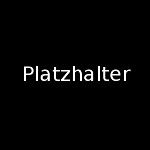
\includegraphics[scale=1.0]{spacer}
		\caption{Modellszene im GUI}
		\label{fig.modscene}
	\end{center}
	%\vspace*{-8mm}
\end{figure}

\red[CAD-Modell oder Punktwolke? Textur wahrscheinlich schlecht abzubilden!?\\]

Die grafische Benutzeroberfläche ermöglicht die individuelle Positionierung und Ausrichtung aller Elemente. Zu beachten ist, dass die Pose der Modellumgebung selbst nicht modifiziert werden sollte, da wie in \kapitel{chap.map} beschrieben das Koordinatensystem der Karte dem globalen Koordinatensystem entspricht.\red[einfach zusätzliche Transformation einbauen?] Der Zusammenhang zwischen den Koordinaten der Modellumgebung und der Karte der Lokalisation wäre bei einer Veränderung der Pose nicht mehr gegeben und würde zu einem Fehler in der späteren Visualisierung führen. \red[Die grafische Benutzeroberfläche enthält die Möglichkeit eine Zuweisung der Modellelemente zu den Gruppen Umgebung und Objekt vorzunehmen, wodurch die Möglichkeiten zur Modifikation der Elemente entsprechend eingeschränkt oder freigegeben werden.]
\red[ Objekteigenschaft bool static um Zugehörigkeit zur Map bzw. globalen Koordinaten zu signalisieren. Eigentlich irrelevant in dieser Beschreibung oder?\\]

\red[Bilder für Modellumgebung und Modellobjekte (z.B. Steckdosen, Leitungen)\\]

\section{Ermittlung der Projektorposition}
Durch die in \abschnitt{chap.perspproj} durchgeführte Kalibrierung des \kps{s} ist die externe Transformation $\tmat{K}{P}$ zwischen der Kamera des Kinect Sensors und dem Projektor bekannt. Die kontinuierlich durchgeführte Lokalisation des \kps{s} liefert die Pose der Kamera innerhalb der Umgebung worüber sich somit auch die Pose des Projektors bestimmen lässt. Ist diese bekannt, kann durch die Kopplung zwischen den Kartendaten der Lokalisation und den verwendeten Modelldaten die Pose des Projektors innerhalb der simulierten Umgebung bestimmt werden:

\begin{equation}
\tmat{M}{P} = \tmat{M}{Odom}\tmat{Odom}{KPS}\tmat{KPS}{P}
\end{equation}

\section{Perspektivische Transformation}
Die perspektivische Abbildung einer 3D Umgebung auf eine 2D Ebene wurde bereits in \kapitel{chap.perspproj} beschrieben. Der Projektor wird eingesetzt um Daten zu visualisieren, welche zwar innerhalb der Modellumgebung, nicht jedoch in der realen Umgebung vorhanden sind. In der Modellumgebung kann der Projektor deshalb als Kamera simuliert werden, wodurch die Abbildung der Perspektive und Visualisierung dieser möglich wird. Die perspektivische Transformation der Modelldaten erfolgt damit basierend auf der durch die Lokalisation bestimmten extrinsischen $\tmat{M}{P}$ und der bei der Kalibrierung ermittelten intrinsischen Transformation $\tmat{SP}{P}$\red[ (bei Kalibrierung nennen!)] des Projektors. Die Abbildung der 3D Modellpunkte auf die 2D pixel der simulierten Kamera wird demnach beschrieben durch:

\begin{equation}
\left(\begin{array}{c}
u'\\
v'\\
w'
\end{array}\right)
= \tmat{SP}{P}(\tmat{M}{P})^{-1}\ve{M}{\tilde{P}} = \tmat{SP}{P}\tmat{P}{M} \left(\begin{array}{c}
X_M\\
Y_M\\
Z_M\\
1
\end{array} \right)
\label{eq.proj_trans}
\end{equation}
%s \cdot \ve{SP}{\tilde{p}} = \tmat{SP}{P}(\tmat{M}{P})^{-1}\ve{M}{\tilde{P}} = \tmat{SP}{P}\tmat{P}{M}\ve{M}{\tilde{P}}

Der durch die Transformation des homogenen 3D-Punktes ermittelte Vektor $[u',v',w']^T$ enthält dabei drei Einträge, welche den in \eq{eq.persp_abb} eingeführten Skalierungsfaktor $s$ enthalten. Um die korrekten Pixelkoordinaten zu ermitteln ist deshalb die Umrechnung der Darstellung des homogenen 2D-Punktes auf einen inversen Streckungsfaktor von $w=1$ erforderlich. Die Pixelkoordinaten des Projektorbildes ergeben sich damit zu:

\begin{equation}
\left(\begin{array}{c}
u\\
v
\end{array}\right)
=
\left(\begin{array}{c}
\nicefrac{u'}{w'}\\
\nicefrac{v'}{w'}
\end{array}\right)
\end{equation}

\abb{fig.perspproj_vtk} zeigt die Abbildung eines Modellobjektes auf die Bildebene des als Kamera simulierten Projektors. \red[Die Bildebene ist dabei wie bereits in \abschnitt{chap.pinhole} beschrieben am Brennpunkt gespiegelt dargestellt.] Bei Generierung der Abbildung ist zu beachten, dass lediglich die Modellelemente sichtbar sind, die mit dem später projizierten Bild visualisiert werden sollen\red[ (im Bild grün hervorgehoben)]. Die Modelldaten aller bereits vorhandenen Strukturen können deshalb ausgeblendet werden, um ungewünschten Überlagerungen zu vermeiden. Um die Projektions- oder Lokalisationsgenauigkeit zu überprüfen können allerdings bewusst Überlagerungen von Modelldaten und realen Strukturen erzeugt werden.

\begin{figure}[!ht]
	\begin{center}
		\includegraphics[scale=1.0]{perspective_03}
		\caption{Perspektivische Abbildung der Modelldaten auf die Sensorebene/Pixeldaten des als Kamera simulierten Projektors, grün hervorgehoben das Objekt, das nicht in der Umgebung vorhanden ist aber projiziert werden soll; Rest ausgrauen oder so?}
		\label{fig.perspproj_vtk}
	\end{center}
	%\vspace*{-8mm}
\end{figure}

\red[Darstellung der Perspektive innerhalb des VTK GUIs]

\section{Projektion}
Nachdem durch die perspektivische Transformation ein Bild der Projektorsicht vorliegt erfolgt die Visualisierung der Modellstrukturen in der realen Umgebung. Da bereits alle nötigen Transformationen des Bildes im Rahmen der perspektivischen Abbildung durchgeführt wurden, kann das vorliegende Bild direkt als Ausgangssignal des Projektors verwendet werden.\\
Ergänzend kann das Bild mit weitere visuellen Informationen versehen werden. \abb{fig.proj_rms} zeigt, wie das Ausgabebild mit einem Rahmen versehen wurde, welcher dem Anwender eine visuelle Rückmeldung über die Güte der Lokalisation basierend auf dem berechneten QMW (siehe \kapitel{chap.globloc}) gibt.\\

\red[Projektion der Sicht des Projektors auf das Modell. Ausblenden des Raumes, sodass nur die gewünschten Strukturen dargestellt werden. Alternativ Raummodell als schwarzes Objekt darstellen.\\]

\begin{figure}[!ht]
	\begin{center}
		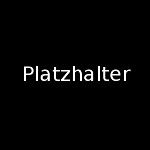
\includegraphics[scale=1.0]{spacer}
		\caption{Visuelle Rückmeldung für den Anwender über die Lokalisationsgüte/Eingeblendete Position im Raum}
		\label{fig.proj_rms}
	\end{center}
	%\vspace*{-8mm}
\end{figure}

\red[Karte einblenden!?]